\documentclass[a4paper,12pt]{report}

\usepackage{alltt, fancyvrb, url}
\usepackage{graphicx}
\usepackage[utf8]{inputenc}
\usepackage{float}
\usepackage{hyperref}

% Questo commentalo se vuoi scrivere in inglese.
\usepackage[italian]{babel}

\usepackage[italian]{cleveref}

\title{Relazione per\\``Programmazione ad Oggetti''}

\author{Nicolò Guerra \and
Emma Leonardi \and 
Filippo Casadei \and
Lorenzo Tagliani}
\date{\today}

\begin{document}

\maketitle

\tableofcontents

\chapter{Analisi}

Bubble Blaster è un gioco della categoria puzzle games, clone del gioco arcade Puzzle Bubble. Il gioco è formato da una schermata
rettangolare in cui vengono create file di bolle colorate che scendono dall'alto. Obiettivo del gioco è utilizzare il cannone
posto in fondo alla schermata per formare gruppi di bolle dello stesso colore e farle così esplodere, cercando di ottenere il maggior
punteggio possibile. La partita è persa se le bolle arrivano in fondo allo schermo.

\section{Requisiti}

\subsubsection{Requisiti funzionali}
\begin{itemize}
	\item All'apertura del gioco verrà mostrata una schermata per la scelta delle modalità di gioco e delle opzioni.
	\item Il gioco dovrà generare una griglia di bolle colorate in maniera casuale.
	\item Il cannone in basso dovrà permettere di sparare bolle generate casualmente, muovendosi angolarmente a destra e sinistra.
	\item Le bolle sparate dal cannone potranno rimbalzare sui muri del campo di gioco se colpiti.
	\item Le bolle dovranno scoppiare alla formazione di gruppi di almeno 3 bolle dello stesso colore adiacenti, facendo cadere eventuali altre bolle sottostanti senza ulteriori sostegni.
	\item Il gioco dovrà dare una schermata di game over se le palline raggiungono il fondo dello schermo.
	\item Il gioco dovrà gestire un punteggio.
\end{itemize}

\subsubsection{Requisiti non funzionali}
\begin{itemize}
	\item Il gioco dovrà fornire una esperienza fluida.
	\item Il gioco dovrà avere musica di sottofondo e effetti sonori per lo scoppio delle bolle e il game over.
\end{itemize}

\subsection{Requisiti facoltativi}
Questi requisiti non sono necessari al funzionamento di base del gioco e per questioni di tempistica potrebbero non essere implementati.
\begin{itemize}
	\item Salvataggio e caricamento della partita
	\item Gestione di una leaderboard con i punteggi migliori
	\item Effetti sonori e musica
	\item Preview della prossima pallina che verrà caricata sul cannone e possibilità di scambiarla con quella caricata
	\item Diversi livelli di difficoltà
	\item Animazioni fluide
	\item Modalità 2 giocatori
\end{itemize}

\section{Analisi e modello del dominio}

L'entità principale in gioco è la Bubble, un insieme di Bubble formano una Grid. Una Grid dovrà poter essere generata in maniera casuale.
Una bolla potrà essere sparata da un cannone, il quale potrà anche decidere di scambiarla con la successiva. Lo scoppio delle bolle dovrà inoltre far incrementare il punteggio.

\begin{figure}[H]
	\centering{}
	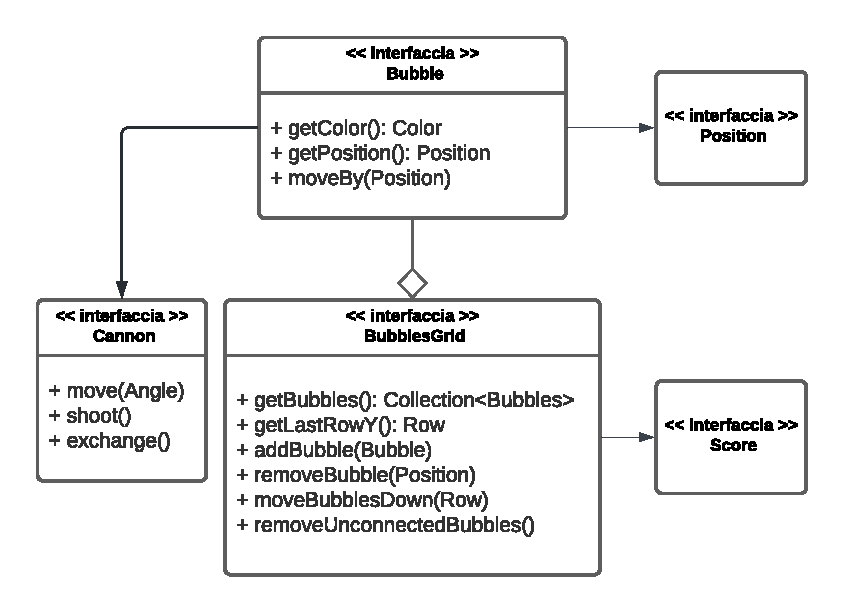
\includegraphics{img/analysis.pdf}
	\caption{UML delle entità che rappresentano il dominio del problema.}
	\label{img:analysis}
\end{figure}

\chapter{Design}

\section{Architettura}

Per questo progetto è stato scelto di fare uso del pattern MVC, che consente di separare in maniera efficace la logica del dominio da quella di visualizzazione e interazione con l'utente.
L'interfaccia principale del Model è rappresentata dal Level che fornisce le informazioni necessarie alla rappresentazione di una partita. La view è nascosta da un interfaccia che non dipende dalla sua
implementazione, in questo modo una sua sostituzione in blocco non dovrebbe comportare modifiche al resto dell'architettura dell'applicazione, questo perché il modello non è in alcun modo a conoscenza
di come venga rappresentato all'esterno.
%
Il punto d'ingresso del Model è il Cannon, che permette al Controller di modificare lo stato del gioco muovendo il cannone e sparando le bolle.
Il tempo del gioco è scandito dal Controller. Il movimento del cannone è invece un evento generato dalla View, che viene passato al Model attraverso il controller e gestito in maniera asincrona.

\begin{figure}[h]
	\centering{}
	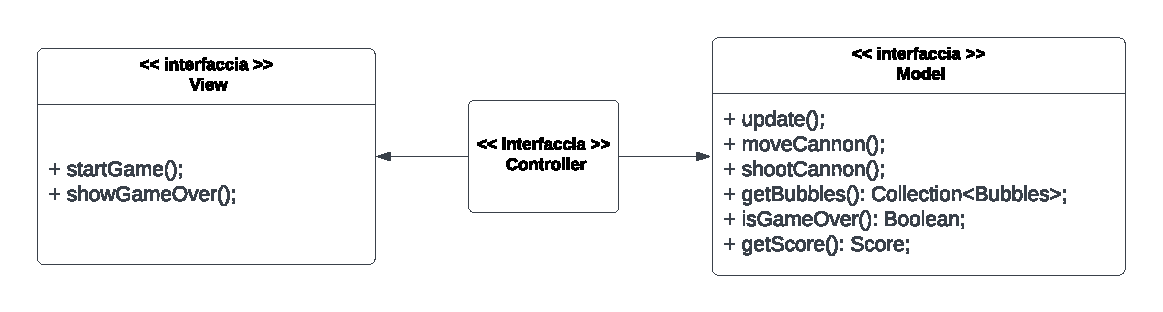
\includegraphics[width=\textwidth]{img/arch.pdf}
	\caption{Schema UML architetturale del gioco. L'interfaccia \texttt{Controller} gestisce il flusso dell'applicazione, mentre la \texttt{View} gestisce l'interazione con l'utente e il \texttt{Model} fornisce le informazioni sul \texttt{Level}.}
\end{figure}

\section{Design dettagliato}
\subsection{Nicolò Guerra}
\subsubsection{Caratteristiche della griglia di bolle}

\begin{figure}[H]
	\centering{}
	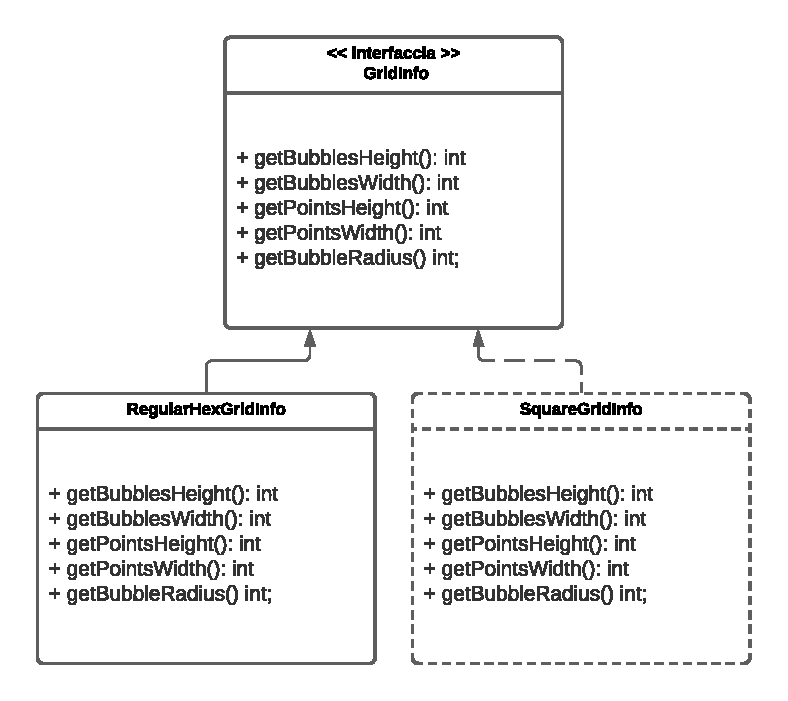
\includegraphics[width=\textwidth]{img/strategy_gridinfo.pdf}
	\caption{Rappresentazione UML dell'oggetto GridInfo}
\end{figure}

\paragraph{Problema} Potenzialmente il gioco può gestire più tipi di griglie diverse per quanto riguarda dimensioni, forme delle caselle e altre caratteristiche, il che può portare a disallineamenti e incoerenze
tra parti diverse del modello, oltre a una difficoltà di rappresentazione delle bolle nello spazio da parte della View, che non conosce griglie o altre entità specifiche del Model.

\paragraph{Soluzione} Le caratteristiche della griglia vengono fornite da una interfaccia di tipo GridInfo implementata come \textit{Strategy}, in questo caso ad esempio la RegularHexGridInfo viene
inizializzata con le dimensioni in bolle della griglia e si occupa autonomamente di effettuare i calcoli necessari per avere una griglia di esagoni regolari. Un'ulteriore implementazione potrebbe essere
ad'esempio una SquareGridInfo che fornisce informazioni per una griglia a celle quadrate.

\subsubsection{Gestione del GameOver}

\begin{figure}[H]
	\centering{}
	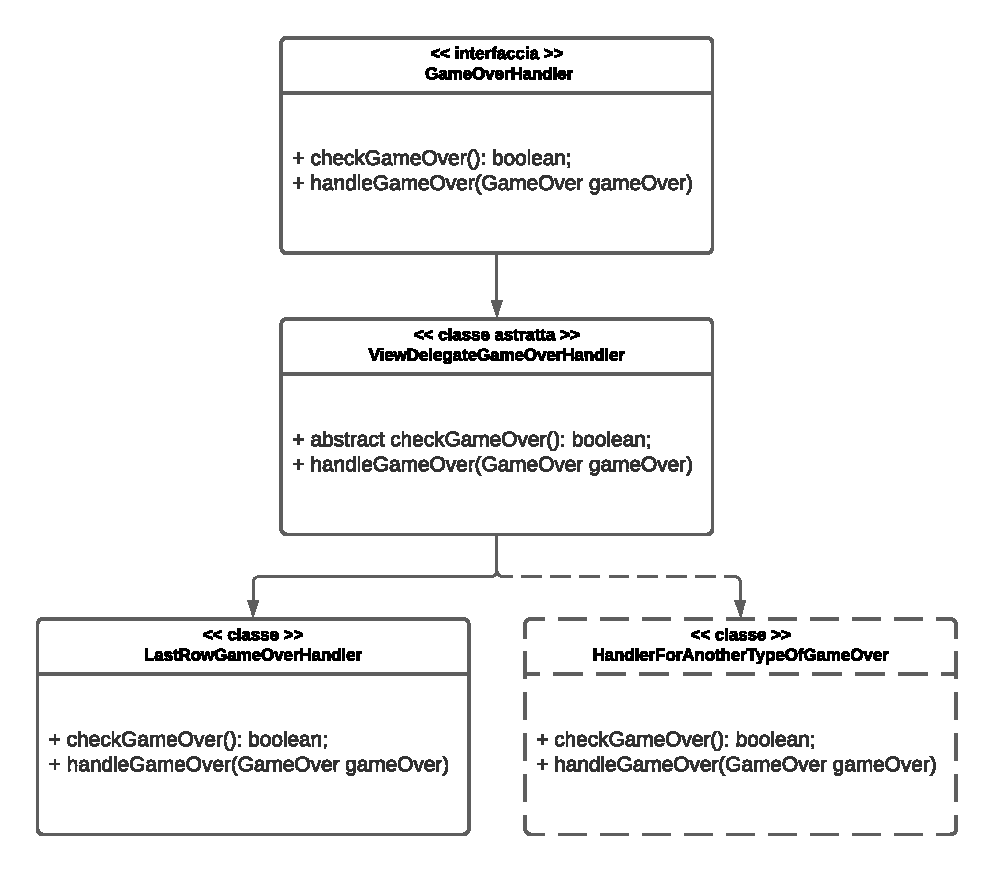
\includegraphics[width=\textwidth]{img/gameover.pdf}
	\caption{Rappresentazione UML del gestore dei GameOver}
\end{figure}

\paragraph{Problema} I GameOver potrebbero essere generati in modi diversi (tempo scaduto, raggiungimento dell'ultima riga...) e voler essere gestiti in maniera diversa.

\paragraph{Soluzione} Un interfaccia GameOverHandler con 2 metodi per controllare se è avvenuto un GameOver e per gestirlo, implementando questa interfaccia è possibile definire quando avviene un GameOver
e come questo venga gestito. Per separare ulteriormente controllo e gestione una classe astratta ViewDelegateGameOverHandler che implementa la gestione passando l'evento di gameover alla View, e con un metodo
astratto per controllare se è accaduto un gameover. Quest'ultimo viene implementato dalla sottoclasse LastRowGameOverHandler, la quale non fa altro che controllare se le bolle nella griglia hanno raggiunto l'ultima
riga.

\subsubsection{Salvataggio su file}

\begin{figure}[H]
	\centering{}
	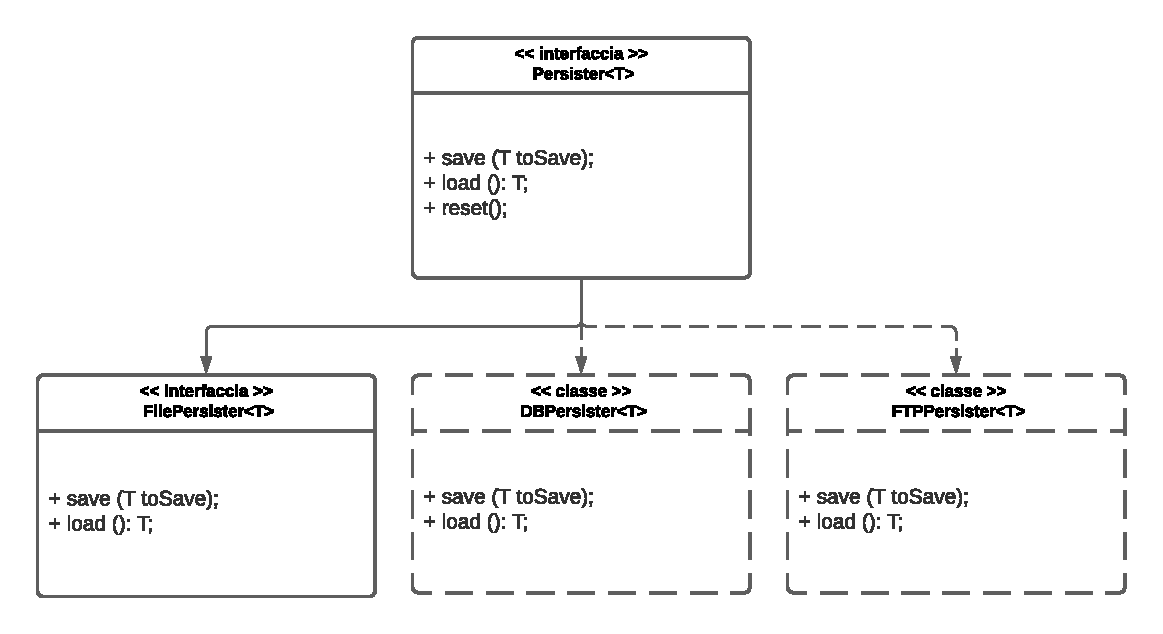
\includegraphics[width=.7\textwidth]{img/persister.pdf}
	\caption{Strategy per un oggetto che salva oggetti}
\end{figure}

\paragraph{Problema} Spesso l'applicazione ha necessita di salvare lo stato di alcuni suoi oggetti per poi recuperarlo in un secondo momento.

\paragraph{Soluzione} Per poter salvare lo stato di oggetti diversi su disco ho creato un interfaccia generica persister che fa da strategy, con un metodo per salvare un oggetto e un metodo per leggerlo.
L'implementazione di questa nasconde all'utilizzatore il modo in cui vengono persistiti. Si possono quindi creare ad esempio diverse implementazioni che salvano su file, su database o in cloud implementando i
metodi read e write. Rispettando la stessa interfaccia le sottoclassi diventano intercambiabili tra di loro.

\subsubsection{Caricamento degli assets della View}

\begin{figure}[H]
	\centering{}
	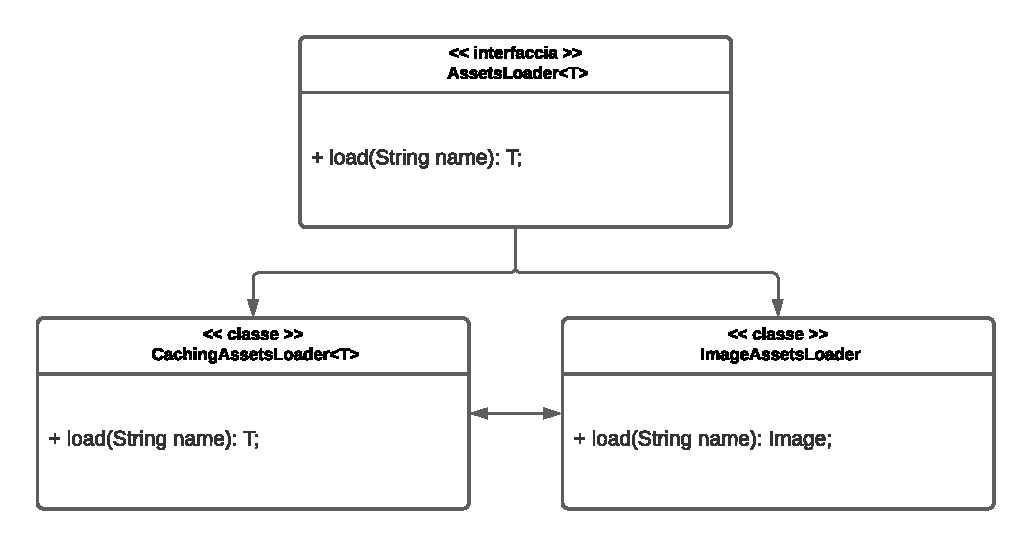
\includegraphics[width=.7\textwidth]{img/assetsloader}
	\caption{Decorator per cache di un assets loader}
\end{figure}

\paragraph{Problema} L'implementazione grafica della View ha bisogno che le vengano forniti gli assets del gioco come le figure delle bolle e del cannone. Deve essere un caricamento efficiente perché gli assets
possono anche essere richiesti più volte al secondo.

\paragraph{Soluzione} Per delegare il caricamento degli assets a un altro componente è stata creata l'interfaccia AssetsLoader che ha un metodo in grado di caricare un assets la cui implementazione
non è specificata. Una classe StandardAssetsLoader carica gli assets dalla cartella resources su richiesta e un CachedAssetsLoader la decora implementando un meccanismo di cache per ridurre gli accessi a disco
e aumentarne l'efficienza. In questo modo è facile riutilizzare il meccanismo di cache per un AssetsLoader che carica altri tipi di assets.

\subsubsection{Gestione del tempo di gioco}

\begin{figure}[H]
	\centering{}
	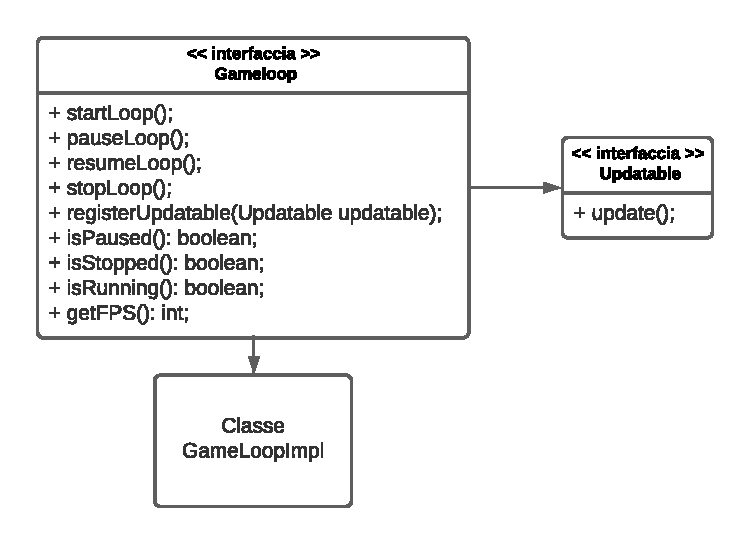
\includegraphics[width=.7\textwidth]{img/gameloop.pdf}
	\caption{UML del Gameloop}
\end{figure}

\paragraph{Problema} Il gioco ha bisogno di essere aggiornato a intervalli regolari, ad esempio per gestire il movimento delle palline o per far ridisegnare la View.

\paragraph{Soluzione} È stato utilizzato il pattern Gameloop, creando un interfaccia che ne definisce le interazioni con il Controller, presso cui altri componenti che implementano Updatable possono registrarsi
per essere aggiornati ad ogni ciclo.

\subsection{Emma Leonardi}
\subsubsection{Gestione del campo di Bolle}

\begin{figure}[H]
	\centering{}
	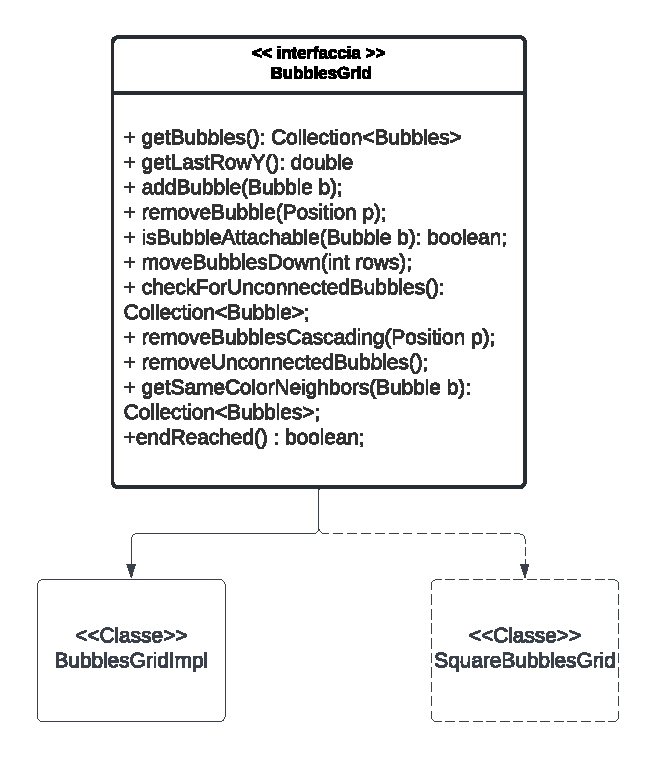
\includegraphics[width=.7\textwidth]{img/bubble_grid.pdf}
	\caption{UML del Gameloop}
\end{figure}

\paragraph{Problema} La griglia di Bolle deve essere indipendente dalla forma delle bolle

\paragraph{Soluzione} Un interfaccia BubblesGrid con metodi che astraggono la forma delle bolle. 
In particolare l'implementazione di BubblesGridImpl è per griglie di esagoni con la punta verso l'alto, 
ma implementando l'interfaccia si possono creare griglie di qualsiasi forma di bolle.

\subsubsection{Gestione di tre valori appaiati}

\begin{figure}[H]
	\centering{}
	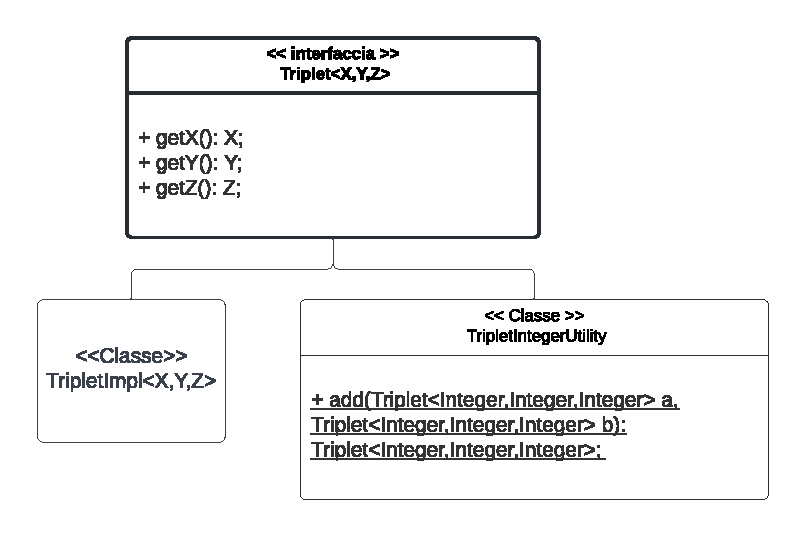
\includegraphics[width=.7\textwidth]{img/triplet.pdf}
	\caption{UML del Gameloop}
\end{figure}

\paragraph{Problema} Nella griglia ho usato coordinate con tre valori e avevo necessità di un oggetto per memorizzarle

\paragraph{Soluzione} Ho creato un'interfaccia generica che supporta qualsiasi tipo di tripletta di valori, poi implementata in una classe generica.
Per poter sommare i valori ho poi creato una classe con metodi statici che fa la somma delle triplette.

\subsection{Filippo Casadei}
\subsubsection{Movimento e collisioni delle bolle}

\paragraph{Problema} Le bolle normalmente sono identificate da un colore e una posizione, ma per potersi spostare hanno bisogno di una velocità per potersi spostare all'interno della griglia di gioco.
Perciò è necessaria un tipo di bolla che può avere una sua velocità.

\paragraph{Soluzione} Per risolvere questo punto è stata modellata una MovingBubble, che estende una bolla normale, che però è caratterizzata da una velocità e da varie operazioni su di essa.

begin{figure}[H]
	\centering{}
	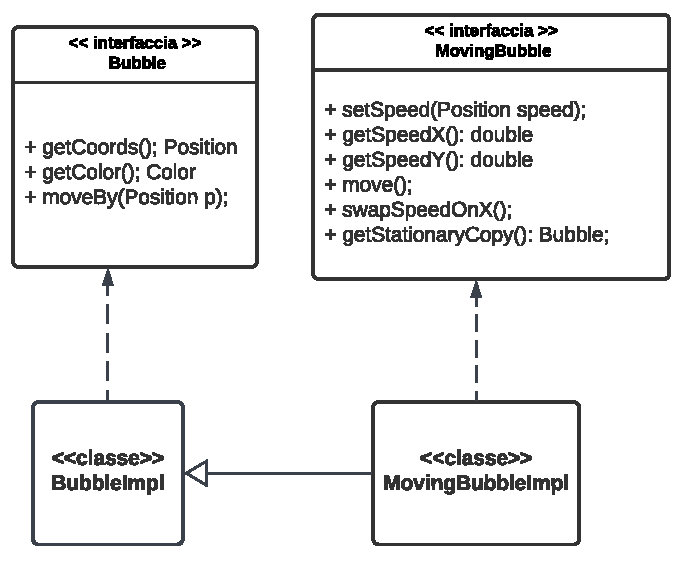
\includegraphics[width=.7\textwidth]{img/movingbubble.pdf}
	\caption{UML della MovingBubble}
\end{figure}

\paragraph{Problema} L'applicazione si comporrà di una griglia di gioco, sulla quale saranno presenti a loro volta una griglia di bolle e la bolla che verrà sparata dal cannone,
quest'ultima potrà muoversi liberamente finchè non verrà a contatto con le bolle già presenti, perciò bisogna controllare che gli spostamenti della bolla in
movimento siano "legali" e che quando questa collida con la griglia di bolle si annetta ad essa.
Inoltre la bolla dovrà poter rimbalzare sui muri laterali facendole cambiare direzione di movimento.

\paragraph{Soluzione} L'entità che gestirà i movimenti della bolla sarà il MovementHandler, quest'ultimo avrà il compito di muovere la bolla solo in posizioni "legali" e nel caso stia per uscire dalla griglia
gestisca il movimento della bolla riposizionandola coerentemente a seconda della sua velocità, facendola rimbalzare se necessario.
Il MovementHandler deve sapere che bolla dovrà controllare, di base non c'è nessuna bolla da controllare.  

begin{figure}[H]
	\centering{}
	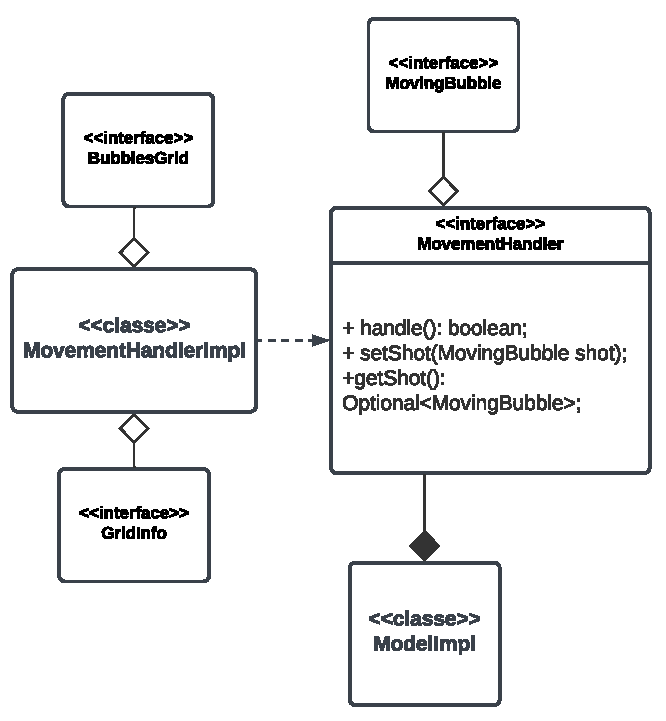
\includegraphics[width=.7\textwidth]{img/movementhandler.pdf}
	\caption{UML del MovementHandler}
\end{figure}

\subsection{Gestione dei livelli}

\paragraph{Problema} L'applicazione dovrà creare ogni volta un nuovo livello che il giocatore potrà giocare, questo livello deve poter essere modificabile in base al livello di sfida che vorrà affrontare
il giocatore. 

\paragraph{Soluzione} Il Level è stato modellato per contenere gli elementi fondamentali di una partita, ovvero è suo compito generare la nuova griglia e il cannone con cui il giocatore interagirà,
inoltre contiene anche il valore numerico del punteggio attuale. Dato che implementa l'interfaccia Serializable è anche possibile salvare lo stato del livello in
qualsiasi momento per poi riprendere da dove si era rimasti.

begin{figure}[H]
	\centering{}
	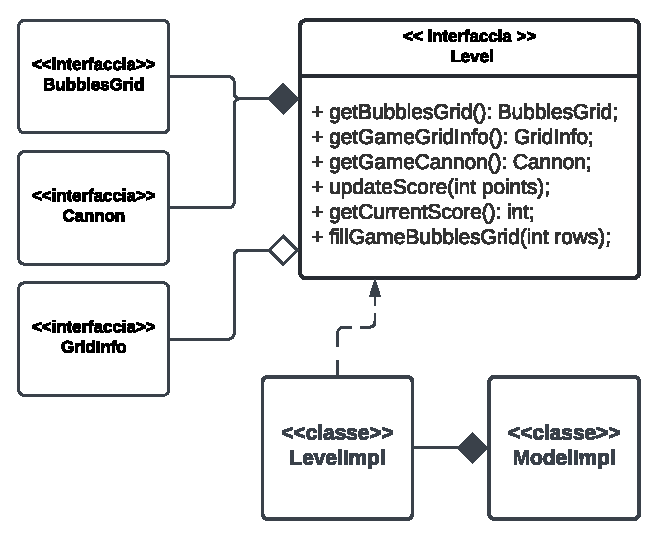
\includegraphics[width=.7\textwidth]{img/level.pdf}
	\caption{UML del Level}
\end{figure}

\subsection{Raffigurazione grafica delle bolle e del campo di gioco}

\paragraph{Problema} L'utente per interagire correttamente con l'applicazione necessita di avere una corretta rappresentazione grafica delle posizioni delle bolle e del cannone,
questa dovrà inoltre esser aggiornata coerentemente durante lo svolgimento della partita.

\paragraph{Soluzione} Per aggiornare continuamente l'intera griglia la view principale farà utilizzo del CanvasDrawer, il quale ha il compito di ridisegnare ad ogni tick 
ogni elemento di gioco, per fare ciò delega il compito di disegnare le bolle, sia quelle della griglia sia quella in movimento, ad un BubbleDrawer, mentre il compito
di disegnare il cannone alla giusta angolazione è delegato ad un CannonDrawer.

begin{figure}[H]
	\centering{}
	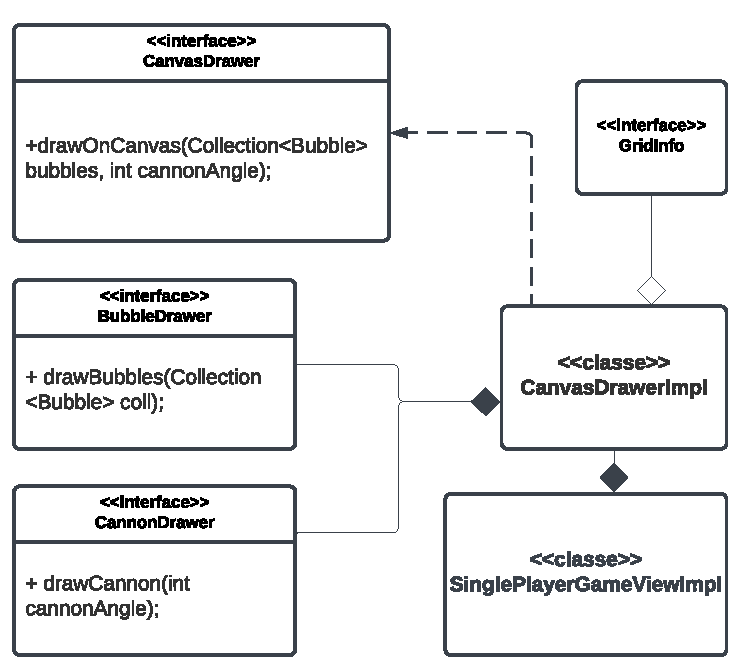
\includegraphics[width=.7\textwidth]{img/drawers.pdf}
	\caption{UML del CanvasDrawer}
\end{figure}

\chapter{Sviluppo}
\section{Testing automatizzato}

Abbiamo usato JUnit 5 per fare test automatici delle classi.

Il testing automatizzato è un requisito di qualunque progetto software che si rispetti, e consente di verificare che non vi siano regressioni nelle funzionalità a fronte di aggiornamenti.
%
Per quanto riguarda questo progetto è considerato sufficiente un test minimale, a patto che sia completamente automatico.
%
Test che richiedono l'intervento da parte dell'utente sono considerati \textit{negativamente} nel computo del punteggio finale.

\subsection*{Elementi positivi}

\begin{itemize}
	\item Si descrivono molto brevemente i componenti che si è deciso di sottoporre a test automatizzato.
	\item Si utilizzano suite specifiche (e.g. JUnit) per il testing automatico.
	\item Se sono stati eseguiti test manuali di rilievo, si elencano descrivendo brevemente la ragione per cui non sono stati automatizzati. Ad esempio, se tutto il team sviluppa e testa su uno stesso sistema operativo e si sono svolti test manuali per verificare, ad esempio, il corretto funzionamento dell'interfaccia grafica o di librerie native su altri sistemi operativi, può avere senso menzionare la cosa.
\end{itemize}

\section{Metodologia di lavoro}

Per lavorare in parallelo su parti diverse del software abbiamo iniziato definendo le interfacce principali dell'applicazione, per poi procedere a sviluppare ognuno a valle delle interfacce che costituivano la sua
parte di progetto. Abbiamo utilizzato branch separati per le feature effettuando il merge sul main alla conclusione di ogni parte di progetto.

\subsection{Nicolò Guerra}

In questo progetto i miei compiti sono stati:
\begin{itemize}
	\item Gestire l'avvio dell'applicazione e la connessione tra i componenti MVC (package bbblast.application)
	\item Gameover (package bbblast.controller.gameover)
	\item Tempo di gioco (package bbblast.controller.gameover)
	\item Informazioni sulla griglia (GridInfo e RegularHexGridInfo nel package bbblast.model)
	\item Persistenza (package bbblast.utils.persister)
	\item Menu principale (package bbblast.utils.menu)
	\item View per le opzioni (package bbblast.view.options)
	\item Caricamento degli assets (package bbblast.view.singleplayer.assetsloader)
\end{itemize}

\subsection{Emma Leonardi}

In questo progetto i miei compiti sono stati:
\begin{itemize}
	\item Gestire il comportamento di Griglie di bolle (package bbblast.model BubblesGrid e BubblesGridImpl)
	\item Bolle statiche (package package bbblast.model Bubble e BubbleImpl)
	\item Comportamento del cannone (package bbblast.model Cannon e CannonImpl)
	\item Grafica del cannone (package bblast.view.singleplayer CannonDrawerImpl e CannonDrawer)
	\item Triplette di valori (package bbblast.utils Triplet, TripletImpl )
	\item Somma di Triplette di valori interi (package bbblast.utils TripletIntegerUtility)
\end{itemize}

\subsection{Filippo Casadei}
In questo progetto i miei compiti sono stati:
\begin{itemize}
	\item Bolle dinamiche (MovingBubble e MovingBubbleImpl, package bbblast.model)
	\item Gestione del movimento e delle collisioni (MovementHandler e MovementHandlerImpl, package bbblast.model)
	\item Divisione in punti (Position e PositionImpl, package bbblast.utils)
	\item Grafica delle bolle (BubbleDrawer e BubbleDrawerImpl, package bbblast.view.singleplayer)
	\item Disegnare la grafica di gioco (CanvasDrawer e CanvasDrawerImpl, package bbblast.view.singleplayer)
	\item Creazione del livello di gioco (Level e LevelImpl, package bbblast.model.level)
\end{itemize}

\section{Note di sviluppo}

\subsection{Nicolò Guerra}
\begin{itemize}
	\item Progettazione di classi generiche
	\item Lambda expressions
	\item Stream
	\item Optional
	\item JavaFX
	\item Thread
\end{itemize}

\subsection{Emma Leonardi}
\begin{itemize}
	\item Stream
	\item Progettazione di classi generiche
	\item Lambda expressions
	\item JavaFX
\end{itemize}
Per la gestione delle coordinate su tre assi ho usato lo pseudocodice di Amit Patel \url{https://www.redblobgames.com/grids/hexagons/} e ho usato sempre il suo codice per cercare gli esagoni vicini.

\chapter{Commenti finali}

In quest'ultimo capitolo si tirano le somme del lavoro svolto e si delineano eventuali sviluppi
futuri.

\section{Autovalutazione e lavori futuri}

\subsection{Nicolò Guerra}

Non sono soddisfatto del progetto che abbiamo svolto. Purtroppo abbiamo avuto diversi problemi già a partire dalla parte di design generale dell'applicazione, complice anche l'inesperienza essendo la prima
volta che ognuno di noi portava avanti un progetto che tutto sommato comincia ad avere dimensioni importanti. Ci sono stati alcuni problemi anche nella coordinazione interna del team, e sicuramente questo
non ha influito positivamente sul risultato finale. Probabilmente avremmo dovuto iniziare scegliendo un progetto diverso da sviluppare e una divisone di compiti diversa, cosa che purtroppo non potevamo sapere
prima di iniziare il progetto. Avremmo dovuto inoltre soffermarci meglio sulle interazioni tra le diverse parti del software. Sono aspetti a cui starò molto più attento una prossima volta.

\subsection{Emma Leonardi}

Sono soddisfatta del mio lavoro individuale, ma non del progetto in totale. Ci sono stati parecchi problemi sulle parti del codice in comune, 
perchè ci sono stati dei problemi di comunicazione e incomprensioni, spesso dovute a una prima fase di design poco precisa. Questo mi ha rallentato nello sviluppo della mia parte di progetto e a tratti ha costretto a riscrivere parti di codice frutto di aspettative diverse di implementazione. 
Non ha aiutato la coordinazione del progetto anche l'inesperienza, che ci ha fatto sottovalutare alcuni aspetti che si sono rivelati problemi implementativi. 
In futuro cercherò di spiegarmi meglio sulle caratteristiche del software prodotto da me e comunicare meglio con i miei compagni di progetto. 

\subsection{Filippo Casadei}
Non sono soddisfatto di come è stato svolto il progetto. Sin dall'inizio della progettazione ci sono state numerose incomprensioni, che hanno portato a dover discutere più volte punti già trattati e capire come risolvere i problemi generati,
rallentando di molto il lavoro di tutti i componenti. A causa di questi problemi a cui si aggiunge anche l'inesperienza di lavorare in progetti più complessi con un team di sviluppo il risultato finale non si può 
assolutamente considerare un buon progetto. Sicuramente però è stata un'esperienza formativa considerando che da ogni sbaglio commesso si è potuto comprendere come sarebbe stato meglio agire, ad esempio una miglior comunicazione
iniziale tra i membri definidendo più nello specifico gli aspetti dell'applicazione ed una miglior suddivisione dello sviluppo del software. 

\section{Difficoltà incontrate e commenti per i docenti}
\subsection{Nicolò Guerra}
Sicuramente la caratteristica che ho apprezzato del corso è la disponibilità dei docenti, le correzioni in laboratorio allo svolgimento di ogni esercizio risultano molto utili per migliorare la tecnica.
Sarebbe interessante approfondire meglio la parte di analisi di dominio di un problema e di design di una soluzione, al di la di quella che è la programmazione Java, che forse è più semplice da capire.

\subsection{Emma Leonardi}
Mi è piaciuta la struttura del corso, i laboratori e l'attenzione dei docenti verso gli studenti. 
Ho trovato di difficile comprensione gli aspetti di Programmazione ad Oggetti avanzati, come Stream e Pattern e avrei voluto gli si fosse dedicato più tempo.

\subsection{Filippo Casadei}
Il corso è stato molto interessante e i docenti hanno avuto la capacità di motivare l'interesse verso la materia e i laboratori si son rivelati esser di grande aiuto per i temi trattati nelle lezioni teoriche.
L'unico punto da me non ben compreso sono gli aspetti riguardanti i pattern, il loro utilizzo e come riconoscere la necessità di utilizzarli.

\appendix
\chapter{Guida utente}

Capitolo in cui si spiega come utilizzare il software. Nel caso in cui il suo uso sia del tutto
banale, tale capitolo può essere omesso.
%
A tal riguardo, si fa presente agli studenti che i docenti non hanno mai utilizzato il software
prima, per cui aspetti che sembrano del tutto banali a chi ha sviluppato l'applicazione possono non
esserlo per chi la usa per la prima volta.
%
Se, ad esempio, per cominciare una partita con un videogioco è necessario premere la barra
spaziatrice, o il tasto ``P'', è necessario che gli studenti lo segnalino.

\subsection*{Elementi positivi}

\begin{itemize}
	\item Si istruisce in modo semplice l'utente sull'uso dell'applicazione, eventualmente facendo uso di schermate e descrizioni.
\end{itemize}

\subsection*{Elementi negativi}
\begin{itemize}
	\item Si descrivono in modo eccessivamente minuzioso tutte le caratteristiche, anche minori, del software in oggetto.
	\item Manca una descrizione che consenta ad un utente qualunque di utilizzare almeno le funzionalità primarie dell'applicativo.
\end{itemize}

\chapter{Esercitazioni di laboratorio}

In questo capitolo ciascuno studente elenca gli esercizi di laboratorio che ha svolto
(se ne ha svolti),
elencando i permalink dei post sul forum dove è avvenuta la consegna.

\subsection{Nicolò Guerra}
\begin{itemize}
	\item Laboratorio 07: \url{https://virtuale.unibo.it/mod/forum/discuss.php?d=88829#p137443}
	\item Laboratorio 08: \url{https://virtuale.unibo.it/mod/forum/discuss.php?d=89272#p138741}
\end{itemize}

\subsection{Emma Leonardi}
\begin{itemize}
	\item Laboratorio 05: \url{https://virtuale.unibo.it/mod/forum/discuss.php?d=87881#p135211}
	\item Laboratorio 06: \url{https://virtuale.unibo.it/mod/forum/discuss.php?d=87880#p135213}
	\item Laboratorio 07: \url{https://virtuale.unibo.it/mod/forum/discuss.php?d=88829#p136445}
	\item Laboratorio 08: \url{https://virtuale.unibo.it/mod/forum/discuss.php?d=89272#p138799}
	\item Laboratorio 09: \url{https://virtuale.unibo.it/mod/forum/discuss.php?d=90125#p138800}
	\item Laboratorio 10: \url{https://virtuale.unibo.it/mod/forum/discuss.php?d=91128#p139973}
\end{itemize}

\bibliographystyle{alpha}
\bibliography{13-template}

\end{document}